\documentclass[12pt]{report}

\usepackage[utf8]{inputenc}
\usepackage[T1]{fontenc}
\usepackage{listings}
\lstset{breaklines=true}
\usepackage[left=2cm,right=2cm,top=2cm,bottom=2cm]{geometry}
\usepackage[frenchb.ldf]{babel}
\usepackage{graphicx}

\title{Scanner Nmap Python}
\author {\bf Auteur\\\\
		Aurélien Bourillon\\
		Valentin Chaigneau\\
		Raphaël Dupin\\\\\\
		\bf Superviseur\\\\
		Nicolas Greneche\\\\\\\\}
\date{23/01/2017}

\begin{document}
\maketitle
\section*{Introduction}
	\paragraph{}
	Dans les entreprises, l'administration d'un parc informatique n'est pas une tâche facile. Les parcs sont de plus en plus grand et un administrateur réseau aura bien du mal à savoir quels services sont présent dans son parc. C'est pourquoi, dans le cadre de nos études, on nous a proposé de réaliser un scanner réseau permettant de connaître rapidement quels sont les services présent dans un parc informatique.	Le principe de ce scanner est assez simple. Il devra scanner un réseau donné pour enregistrer dans une base de données différentes informations que nous verrons plus tard. Ce scanner sera sous la forme d'un daemon pour faciliter l'automatisation. Ces résultats seront visible via un SiteWeb qui permettra de générer un fichier de règles pour un firewall.
	\paragraph{}
	Ce rapport présentera les outils utilisés à savoir NMAP et l'API Python de NMAP. Nous exposerons ce que NMAP permet et pourquoi le choix du langage python est interressant dans ce cas. Nous verrons ensuite l'installation et la configuration du daemon via les fichiers fourni. 
\tableofcontents
\part{Présentation du contexte}
	\chapter{NMAP}
		\paragraph{}
			NMAP ("Network Mapper") est un outil open source d'exploration réseau et d'audit de sécurité. Il permet l'analyse de plage réseau ou d'une machine précise. Grâce à des paquets IP bruts (raw packets), il peut déterminer de nombreuses informations concernant les services (port, nom du service, version...), mais aussi concernant la machine. En effet, NMAP permet de connaitre l'OS de la machine que nous analysons.
			\begin{lstlisting}[caption=Scan NMAP, captionpos=b]
# nmap -A -T4 81.194.43.80

Starting Nmap 7.40 ( https://nmap.org ) at 2017-01-25 13:17 CET
Nmap scan report for monitor.univ-paris13.fr (81.194.43.80)
Host is up (0.022s latency).
Not shown: 997 filtered ports
PORT      STATE  SERVICE VERSION
80/tcp    open   http    Apache httpd 2.2.8 ((Ubuntu))
|_http-server-header: Apache/2.2.8 (Ubuntu)
|_http-title: Did not follow redirect to /cacti/
443/tcp   closed https
20031/tcp open   unknown
Device type: general purpose
Running: Linux 2.6.X
OS CPE: cpe:/o:linux:linux_kernel:2.6
OS details: Linux 2.6.15 - 2.6.26 (likely embedded), Linux 2.6.29 (Gentoo)
Network Distance: 13 hops

OS and Service detection performed. Please report any incorrect results at https://nmap.org/submit/ .
Nmap done: 1 IP address (1 host up) scanned in 39.56 seconds
			\end{lstlisting}
			\paragraph{}
				Sur cet exemple nous pouvons voir que la machine analysée a trois services disponible. HTTP est ouvert sur le port 80, HTTPS closed sur le port 443 et un autre service inconnu sur le port 20031. Il faut savoir que l'état "open" et "closed" sont assez courant mais ce ne sont pas les seuls. En effet, nmap peut voir un service en état "filtered" ou "unfiltered". Voici l'explication pour chacun de ces états :
			\begin{description}
			\item OPEN : Le service de la machine est en écoute sur ce port
			\item CLOSED : Aucun service en écoute sur ce port. Mais il peut s'ouvrir n'importe quand.
			\item FILTERED : Ici NMAP nous indique qu'un dispositif l'a empéché de déterminer si le service est ouvert ou fermé. Cela peut-être dû à un pare-feu par exemple.
			\item UNFILTERED : Ces ports sont particuliés, car ils répondent aux paquets test de NMAP, cependant NMAP ne peut pas déterminer s'ils sont ouverts ou fermés.
			\end{description}
			\paragraph{}
				En bref, NMAP offre de nombreuses possibilités qui peut répondre au projet que nous devons réaliser. Les explications précédentes ne sont qu'une petite partie de ce que peut faire NMAP. Il peut par exemple effectuer du reverse DNS, connaître le type de matériel de la machine ou même retrouver les adresses MAC.
	\chapter{Python}
		\section{Python en bref}
			\paragraph{}
				Python est un langage de programmation créé en 1991, mais baptisé seulement en 2001 (Python Software Foundation). Les informatitiens aiment penser que le nom de ce langage est une référence aux "Monty Python" dont Guido van Rossum était fan. Mais Concrétement qu'est ce que Python ? Tout d'abord il faut savoir que python est un langage facile (bien que son indentation reste un petit casse-tête) à apprendre, mais qui offre de nombreuses possibilités. Les programmes sont appelés script qui ont souvent une seule mission bien précise. Cependant il est possible de réaliser des jeux vidéos, logiciels en tout genre voir même des progiciels (souvent utilisés par les professionnel, ce sont plusieurs logiciels fonctionnant ensemble).
			\paragraph{}
				Ce langage utilise un système de typage automatique. C'est à dire que lors de l'affectation d'une variable, Python va en déduire le typage (int, float, str...). Par exemple voici une suite de commande affectant une variable et dont on affichera le type :
				\begin{lstlisting}[caption=Affectation variable en Python, captionpos=b]
			>>> variable="Bonjour"
			>>> type(variable)
			<type 'str'>
			>>>
				\end{lstlisting}
			\paragraph{}
				Nous pouvons voir sur cet exemple que la variable est affectée à une chaîne de caractère. Python déduira alors son type automatiquement. Mais alors pourquoi utiliser Python dans notre projet ? Comme nous l'avons vu nous pouvons créer des scripts. Ce qui permettra d'automatiser le scan réseau plus facilement. Mais surtout Python à une API qui permet d'interragir avec NAP. C'est ce que nous allons voir maintenant.
		\section{l'API NMAP}
			\paragraph{}
				Dans cette partie nous allons exposer le fonctionnement et l'utilisation de l'API NMAP Python. Pour que cette API fonctionne, NMAP doit être installé sur la machine. Voici la démarche à suivre pour effectuer un scan sur la même machine que tout à l'heure mais en spécifiant une plage de port, mais en Python :
				\begin{lstlisting}[caption=Scan NMAP avec Python, captionpos=b]
>>> import nmap
>>> nm = nmap.PortScanner()
>>> nm.scan("81.194.43.80", "22-443", arguments='-sV')
{'nmap': {'scanstats': {'uphosts': '1', 'timestr': 'Wed Jan 25 14:12:35 2017', 'downhosts': '0', 'totalhosts': '1', 'elapsed': '15.91'}, 'scaninfo': {'tcp': {'services': '22-443', 'method': 'connect'}}, 'command_line': 'nmap -oX - -p 22-443 -sV 81.194.43.80'}, 'scan': {'81.194.43.80': {'status': {'state': 'up', 'reason': 'syn-ack'}, 'hostnames': [{'type': 'PTR', 'name': 'monitor.univ-paris13.fr'}], 'vendor': {}, 'addresses': {'ipv4': '81.194.43.80'}, 'tcp': {80: {'product': 'Apache httpd', 'state': 'open', 'version': '2.2.8', 'name': 'http', 'conf': '10', 'extrainfo': '(Ubuntu)', 'reason': 'syn-ack', 'cpe': 'cpe:/a:apache:http_server:2.2.8'}, 443: {'product': '', 'state': 'closed', 'version': '', 'name': 'https', 'conf': '3', 'extrainfo': '', 'reason': 'conn-refused', 'cpe': ''}}}}}
				\end{lstlisting}
			\paragraph{}
				Nous avons tout d'abord importé la libraire nmap, pour ensuite affecter une variable au PortScanner() de NMAP. Pour finir par lancer un scan en spécifiant une IP, une plage de port et des arguments NMAP. Mais finalement que fait l'API ? En fait, rien d'extraordinaire, si nous regardons les processus en cours lors de l'execution de la commande :
				\begin{lstlisting}
$ ps aux | grep nmap
kungfury  3061 12.0  0.3  74708 31304 pts/1    S+   14:13   0:00 nmap -oX - 81.194.43.80 -p 22-443 -sV
				\end{lstlisting}
			\paragraph{}
				Nous pouvons remarquer que le script fait appel à NMAP avec l'option "-oX". Cette option permet de formater la sortie du scan au format XML. Une fois cette sortie récupérée, l'API n'a plus qu'à ranger les informations dans une structure que nous pourrons interroger par la suite. Elle est d'ailleur affichée en sortie dans l'exemple de scan NMAP avec Python. Mais cette fonctionnalité ne sort pas seulement une structure. Nous le verrons plus en détail lorsque nous parlerons de notre solution final, mais nous pouvons faire appel à différentes fonction pour nous simplifier la vie. Voici un exemple qui permet de récupérer le nom d'un service sur une machine donnée.
				\begin{lstlisting}[caption=Récupération du nom d'un service, captionpos=b]
>>> nm.all_hosts()
['81.194.43.80']
>>> nm['81.194.43.80'].all_protocols()
['tcp']
>>> nm['81.194.43.80']['tcp'].keys()
[80, 443]
>>> nm['81.194.43.80']['tcp'][80]['name']
'http'
				\end{lstlisting}
		\section{L'API MYSQL}
			\paragraph{}
				Nous l'avons vu en introduction, les résulatats trouvés par le script python seront stockés dans une base de données. Nous allons exposer ici comment dialoguer avec une base de données MYSQL en Python. Le paquet "python-connector" est necessaire pour effectuer l'exemple suivant :
				\begin{lstlisting}[caption=Connexion à une base de données et insertion de données, captionpos=b]
>>> unnom="KungFury"
>>> import mysql.connector
>>> bdd = mysql.connector.connect(host='IP_BDD',user='nom_user',password='pass_user', database='nom_BDD')
>>> cursor = bdd.cursor()
>>> cursor.execute("""INSERT INTO exemple (nom) VALUES(%s)""", (unnom))
>>> bdd.commit()
				\end{lstlisting}
			\paragraph{}
				Dans cet exemple, nous nous sommes connectés à une base de données grâce à "mysql.connector". Une fois connecté nous récupérons un cursor qui permettra d'effectuer les requêtes SQL. Une fois la requête voulu mis en attente grâce au curseur, il suffit de commit avec l'objet "mysql.connector". Il est possible de faire plusieurs requêtes SQL avant de commit. Maintenant, voici la procédure à suivre pour récupérer des résultats (nous gardons les mêmes variables que précédemment) :
				\begin{lstlisting}[caption=Récupérationd de données, captionpos=b]
>>> query = 'SELECT ID FROM table WHERE nom = '+unnom
>>> cursor.execute(query)
>>> result = cursor.fetchone()
				\end{lstlisting}
			\paragraph{}
				Ici, nous avons récupéré un résultat grâce à la fonction "fetchone()". Il aurait été possible de récupérer plus de résultats grâce à la fonction "fetchall()". Nous aurions alors eu une liste de résultats.
	\chapter{Le projet}
		\paragraph{}
			Nous venons de voir les différents outils que nous allons utiliser pour réaliser le projet. Nous allons maintenant exposer le sujet de ce projet. Comme dit en introduction le but est de faire un scanner qui enregistrera les résultats dans une base de données. Nous avons pour consigne de récupérer les informations suivantes :
			\begin{itemize}
				\item Pour les machines :
					\begin{itemize}
						\item L'adresse IP
						\item Le FQDN (Fully Qualified Domain Name) : Position absolue d'un noeud dans une arborescence DNS
						\item La dernière fois que la machine a été vu
					\end{itemize}
				\item Pour les services :
					\begin{itemize}
						\item Le protocole
						\item Le port
						\item Le nom du service
						\item Son état
						\item La banner
						\item La version
						\item La dernière fois que le service a été vu
					\end{itemize}
			\end{itemize}
		\paragraph{}
			Un aspect important de l'administration d'un parc informatique est de savoir qui est présent sur le réseau et surtout à quel moment. C'est pourquoi nous devons récupérer la date où le scanner voit la machine ou le service. Si nous voyons un service ouvert à un telle date et que depuis ce service n'existe plus, nous pouvons nous poser des questions. Quoi qu'il en soit pour voir les machines de façon régulière le script doit être automatisé. C'est pourquoi nous allons en faire un daemon pour qu'il puisse agir en permanence. Uns fois ces tâches effectuée, les résultats seront visibles depuis une interface WEB. Ainsi, nous pourrons voir d'un coup d'oeil voir les machines et les services présent. Il y aura même la possibilité de générer un fichier de règles en fonctions des services que nous voulons ou non. Si par exemple sur une machine un service inconnu est en écoute sur le port 12345, l'administrateur réseau pourra selectionner le fait qu'il ne veut pas le laisser passer. Le site générera un fichier de règles de pare-feu.
\part{Présentation et installation de la solution}
	\chapter{Le script d'installation}
		\paragraph{}
			Pour l'installation de notre solution nous proposons un script qui installera toute la partie BDD (dont nous verrons la structure plus tard) et daemon. Nous avons au départ donc deux fichiers à savoir "install\_scanner.sh" et "jajscan.py" dont nous parlerons plus tard. Le script d'installtion peut recevoir plusieurs arguments qui sont les suivants :
			\begin{description}
				\item install : Permet l'installation totale de la solution
				\item reinstall : Supprimera tout les fichiers de configurations, d'interraction avec la BDD, le daemon et les logs. Puis relancera l'installation.
				\item clearbdd : Permet de vider les tables créées à l'installation
				\item unistall : Supprimera la totalité de la solution et supprimera les tables dans la BDD.
			\end{description}
		\paragraph{}
			Pour installer la solution il faut néanmoins créer au préalable une Database. L'installateur se chargera de créer les tables. Il suffit pour lancer l'installation de faire comme suit :
			\begin{lstlisting}[caption=Installation, captionpos=b]
# chmod +x install_scanner.sh 
# ./install_scanner.sh install
Creation du dossier de log : /var/log/pythonnmap/
Creation du service...
Adresse de la BDD : 127.0.0.1
Nom de la base : Scanner
Nom utilisateur BDD : scanner_user
Mot de passe BDD : 
Reseau a analyser [0.0.0.0/24] : 192.168.10.0/24
Port a analyser [Port_debut-Port_fin / all] : all
NOTE : En vitesse fast l analyse est moins precise !
Vitesse d analyse [fast/slow] : slow
Voulez-vous recevoir les resultats du scan par mail (SMTP uniquement)? [y/n]n
Creation du fichier de configuration...
Creation des script SQL...
Renseignez un utilisateur disposant des droits CREATE/ALTER sur la table  Scanner
Nom utilisateur : root
Mot de passe :
#
			\end{lstlisting}
		\paragraph{}
			Durant l'installation, un certain nombre de questions sont posées afin de bien configurer le daemon. Suite à cette installation plusieurs dossiers et fichiers sont créé :
			\begin{figure}[ht]
				\begin{center}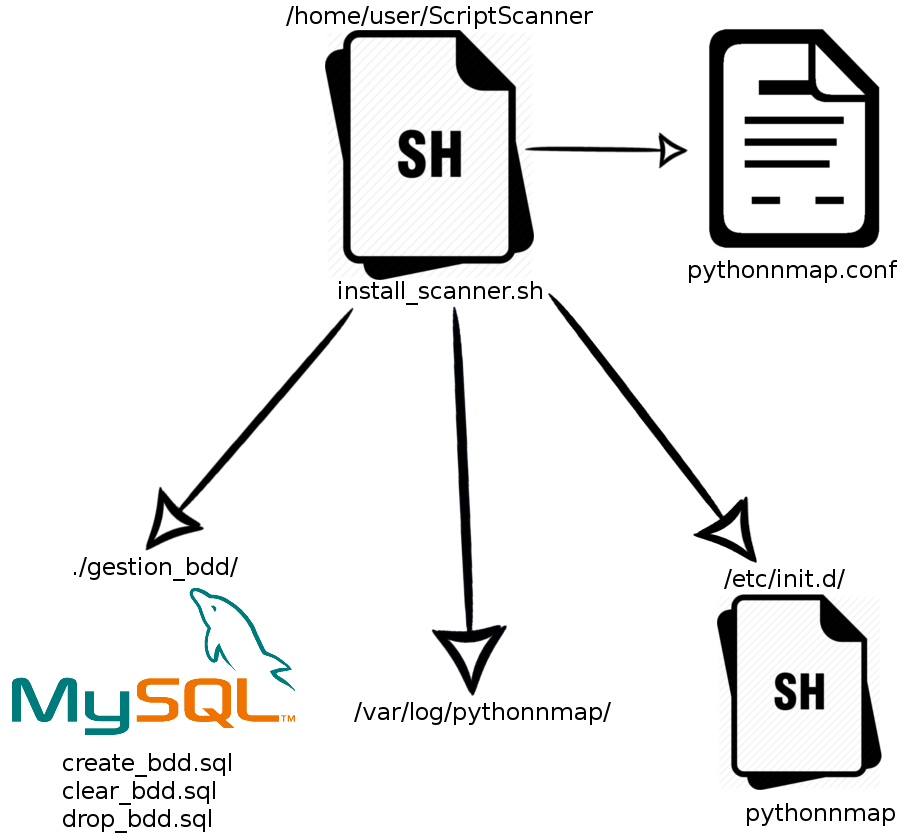
\includegraphics[height=250pt,keepaspectratio]{/home/valentin/Python_scan/Rapport/IMG/Install.png}
				\caption{\label{create_file} Fichiers et dossiers créés suite à l'installation}\end{center}
			\end{figure}
		\paragraph{}
			Comme nous pouvons le voir, l'installation a créé :
			\begin{itemize}
				\item Les fichiers SQL permettant au script d'installation d'interragir avec la BDD
				\item Le dossier où se trouveront les logs du daemon
				\item Le daemon "pythonnmap"
				\item Le fichier de configuration du daemon
			\end{itemize}
		\paragraph{}
			Ce fichier de configuration sera lu par le daemon pour lire les différents paramètres du scan. Ainsi, nous ne sommes pas obligé de reinstaller toute la solution si nous decidons de changer la cible du scan.
			\begin{lstlisting}[caption=Exemple fichier de configuration, captionpos=b]
############# CONFIGURATION SCANNER PYTHON NMAP #############
BDDAddr = 127.0.0.1
BDDName = Scanner
BDDUser = scanner_user
BDDPass = user@pass
Reseau = 192.168.10.0/24
## Format : PortDebut-PortFin ou mettre all pour scanner tout les ports
Port = all
## Format : slow ou fast (le mode fast est moins precis)
Speed = slow
########### CONFIGURATION MAIL SCANNER PYTHON NMAP ###########
## Mettre y pour activer l envoie de mail
Envoimail = n
AddrSend = 
Passmail = 
##Adresse destination format : mail1, mail2, mail3...
AddrDest = 
AddrSMTP = 
PortSMTP =

			\end{lstlisting}
		\paragraph{}
			Le daemon offre la possibilité d'envoyer les résultats par mail (nous le verrons en détail plus tard). Dans ce fichier il faudra renseigner les différents paramètres de serveur mail (seulement SMTP). Le paramètre "speed" permet de spécifier si le daemon utilisera les threads NMAP ou non (mode fast pour les utiliser). En sachant que ce mode est moins précis et peut ne pas remonter les résultats demandé.
	\chapter{La base de données}
		\paragraph{}
			Nous l'avons vu durant l'installation, il est necessaire de créer une base de données. Le script d'installation va lui créer les tables qui permettrons de stocker les informations receuilli par le scanner. Il y aura deux tables à savoir une table "machines" et une table "services". Elles seront configurée comme suit :\\
			\begin{table}[h]
			\centering
			\begin{tabular}{|c|c|}
				\hline
					Nom & Type \\
				\hline
				\hline
					mid & int \\
				\hline
					fqdn & text \\
				\hline
					ip & text \\
				\hline
					last\_view & datetime\\
				\hline
			\end{tabular}
			\caption{\label{machines_bdd} Table Machines}
			\end{table}
			\begin{table}[h]
			\centering
			\begin{tabular}{|c|c|}
				\hline
					Nom & Type \\
				\hline
				\hline
					sid & int \\
				\hline
					mid & int \\
				\hline
					proto & text \\
				\hline
					port & int \\
				\hline
					nom\_service & text \\
				\hline
					sate & text \\
				\hline
					banner & text \\
				\hline
					version & text \\
				\hline
					last\_view & datetime \\
				\hline
					manage & int \\
				\hline
			\end{tabular}
			\caption{\label{services_bdd} Table Services}
			\end{table}
		\paragraph{}
			Ces tables sont lié par le "mid" qui est l'ID de la machine. Cette clé étrangère présente dans la table service permet de faire rapidement le lien avec la machine associée. La colonne "manage" est présente pour savoir si le service à été pris en compte par l'utilisateur via l'interface WEB.
	\chapter{Le daemon}
		\paragraph{}
			Nous avons vu l'installation et la base de données qui en découle. Maintenant, nous allons voir le daemon. Dans cette partie nous ne parlerons pas du script Python, mais de comment il est appelé et géré. Lors de la création du daemon, le script a pris en compte les options de l'utilisateur ainsi que le dossier courant. C'est-à-dire qu'il a créé un daemon sur mesure en fonction d'où se trouve le script d'installation et le scanner Python. Le scanner sera appelé avec un argument qui sera le fichier de configuration qui se trouve aussi dans le dossier du script d'installation. Le daemon pourra ainsi être lancé grâce à la commande :
			\begin{lstlisting}
			# service pythonnmap start
			\end{lstlisting}
		\paragraph{}
			Le script Python tourera alors comme un service. Etant donné qu'il possède une boucle infini celui-ci continuera sont execution jusqu'à l'arrêt du service ou de la machine.
\part{Le script Python}
\end{document}